\section{Bartosz Zieliński}

Twierdzenie o odcinkach siecznej i stycznej:
Dane są: prosta przecinająca okrąg w punktach \(A\) i \(B\) oraz prosta styczna do tego okręgu
w punkcie \(C\) Jeżeli proste te przecinają się w punkcie \(P\), to:
\[ |PA| * |PB| = |PC|^2 \]


\begin{figure}[htbp] 
\centering
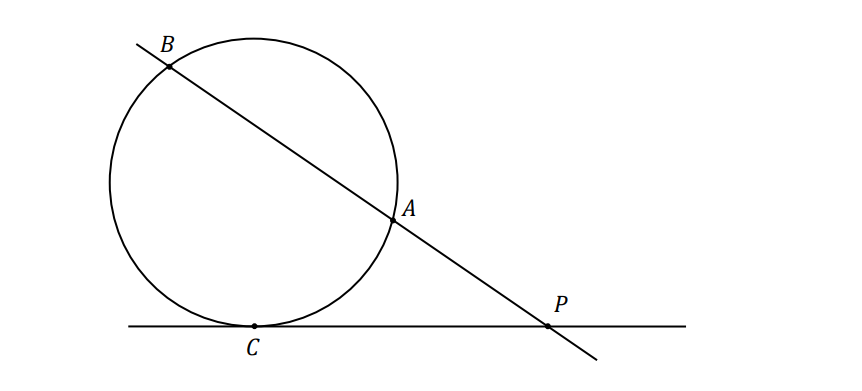
\includegraphics[width=0.6\textwidth]{pictures/123.png}
\caption{\label{fig:123}Obraz}
\end{figure}

Tabelka pokazująca przykładową rozgrywkę w kółko i krzyżyk:

\begin{table}[htbp]
\centering
\begin{tabular}{|l|l|l|}
\hline
X & O & X \\ \hline
X & O & O \\ \hline
O & X & X \\ \hline
\end{tabular}
\label{tab:table_bartek}
\caption{Kolko i krzyzyk}
\end{table}

Lista zakupów:
\begin{enumerate}
\item Mleko,
\item Makaron.
\end{enumerate}
\begin{itemize}
\item Penne,
\item Spaghetti.
\end{itemize}


This is text contained in the \underline{first} paragraph. 
This is text contained in the \emph{first} paragraph. 
This is text contained in the \textbf{first}  paragraph.\par
This is text contained in the second paragraph. 
This is text contained in the second paragraph.
This is text contained in the second paragraph.

To jest odniesienie do twierdzenia o stycznej i siecznej - LINK \ref{fig:123}